
برای Derivation Most Left از راست‌ترین E شروع کرده و عبارت‌های معادل را جایگزین می‎‌کنیم تا به عبارت مورد نظر برسیم:

\setLTR


E {\LARGE $\rightarrow$} EBE  

\hspace{1em}{\LARGE $\rightarrow$} [E]BE   

\hspace{1em}{\LARGE $\rightarrow$} [EBE]BE  

\hspace{1em}{\LARGE $\rightarrow$} [VBE]BE  

\hspace{1em}{\LARGE $\rightarrow$} [aBE]BE 

\hspace{1em}{\LARGE $\rightarrow$} [a!E]BE 

\hspace{1em}{\LARGE $\rightarrow$} [a!V]BE 

\hspace{1em}{\LARGE $\rightarrow$} [a!b]BE 

\hspace{1em}{\LARGE $\rightarrow$} [a!b]@E 

\hspace{1em}{\LARGE $\rightarrow$} [a!b]@[E] 

\hspace{1em}{\LARGE $\rightarrow$} [a!b]@[V] 

\hspace{1em}{\LARGE $\rightarrow$}	[a!b]@[a] 



\setRTL
برای Derivation Most Right
از راست‌ترین E شروع کرده و عبارت‌های معادل را جایگزین می‎‌کنیم تا به عبارت مورد نظر برسیم:

\setLTR


E {\LARGE $\rightarrow$} EBE  

\hspace{1em}{\LARGE $\rightarrow$}  EB[E]

\hspace{1em}{\LARGE $\rightarrow$}  EB[V]

\hspace{1em}{\LARGE $\rightarrow$} EB[a]

\hspace{1em}{\LARGE $\rightarrow$}  E@[a]

\hspace{1em}{\LARGE $\rightarrow$} [E]@[a]

\hspace{1em}{\LARGE $\rightarrow$} [EBE]@[a]

\hspace{1em}{\LARGE $\rightarrow$} [EBV]@[a]

\hspace{1em}{\LARGE $\rightarrow$} [EBb]@[a]

\hspace{1em}{\LARGE $\rightarrow$} [E!b]@[a]

\hspace{1em}{\LARGE $\rightarrow$} [V!b]@[a]

\hspace{1em}{\LARGE $\rightarrow$} [a!b]@[a]
\pagebreak
\setRTL

حال درخت Parse را رسم می‌کنیم:

\begin{figure}[htbp]
	\centering
	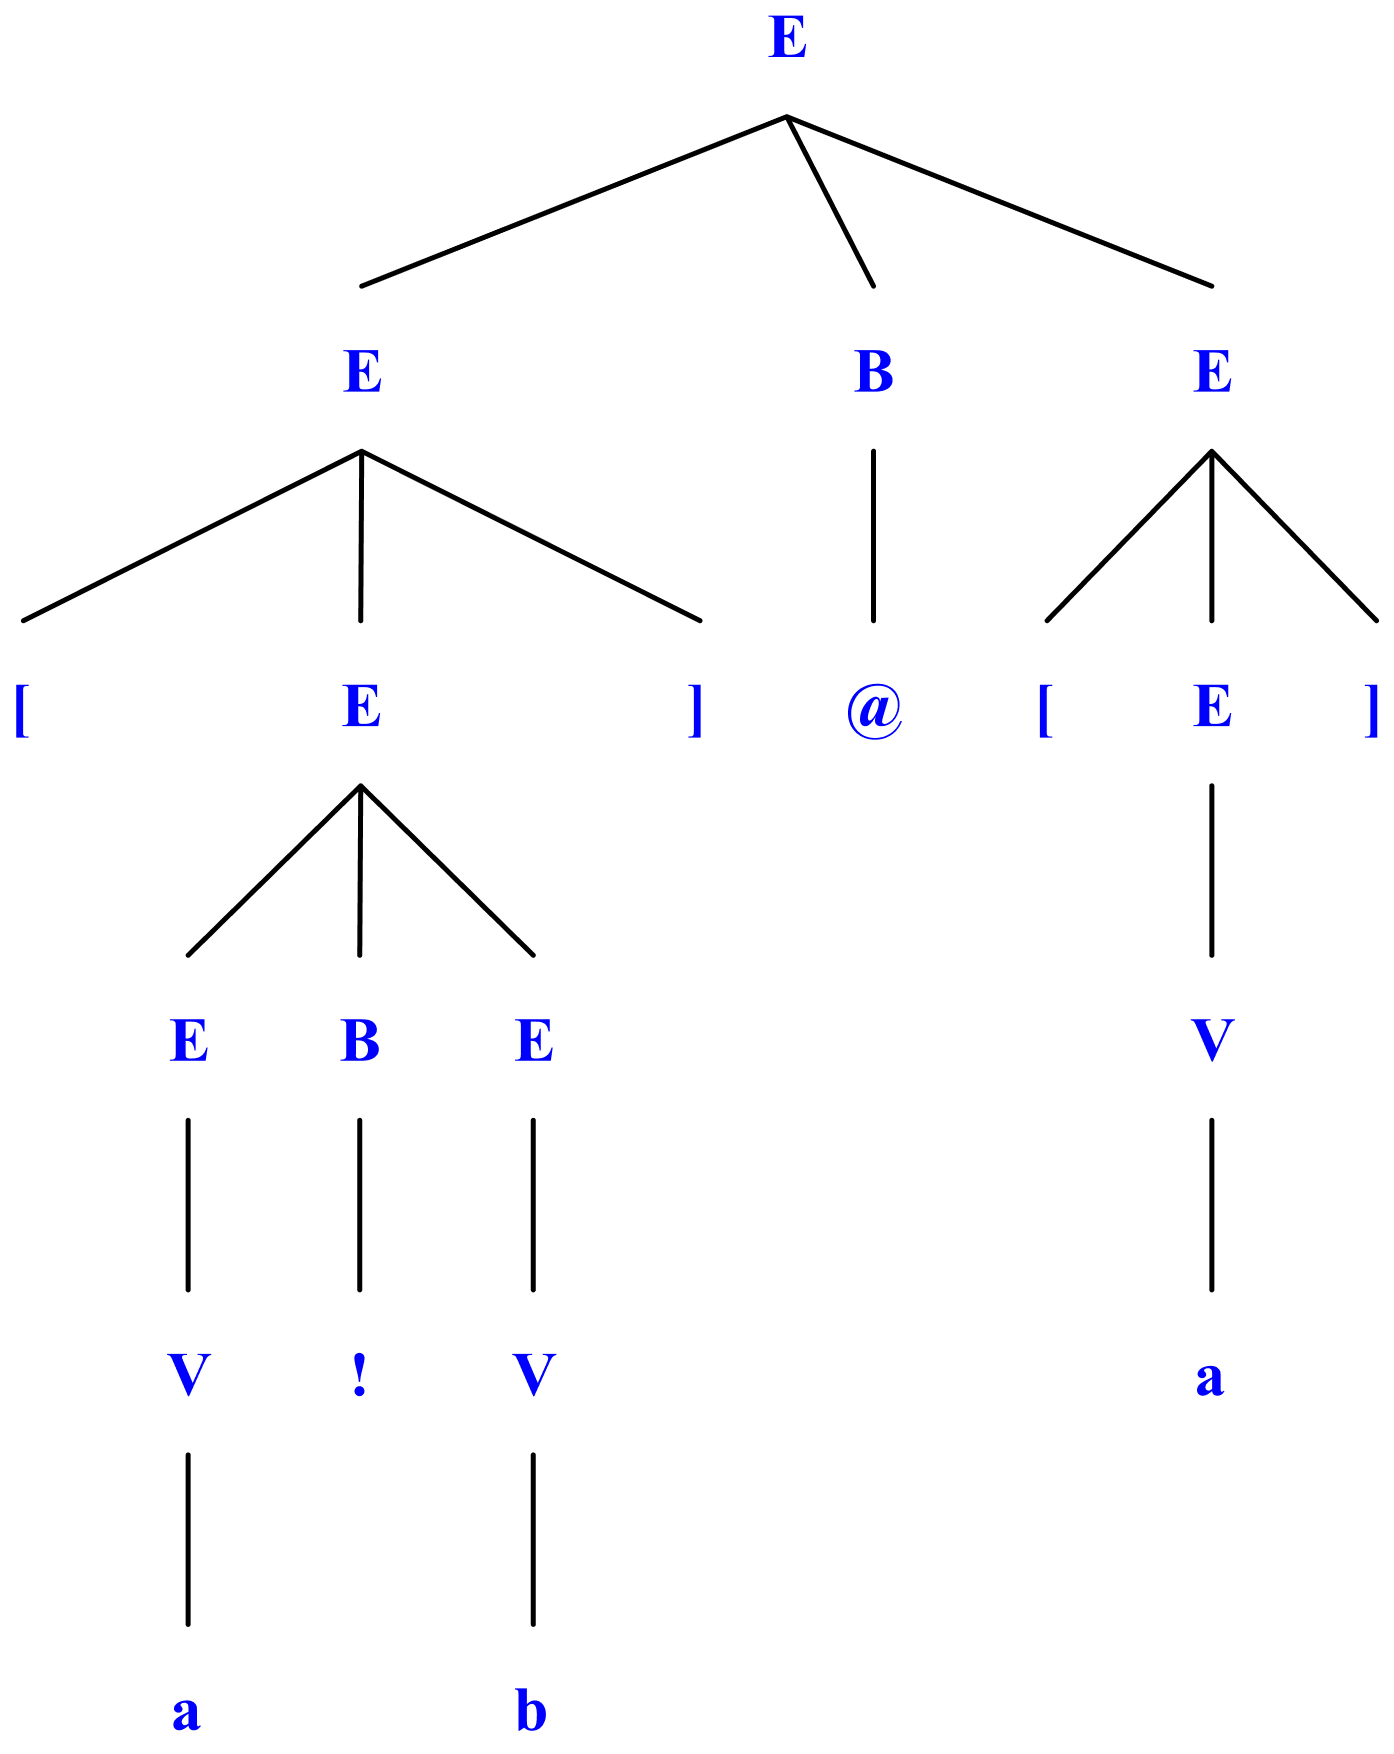
\includegraphics[width=0.5\textwidth]{1.png}
	
\end{figure}


